% One serial line, two consumers, and the thing that makes that work.
%
% The drawing exists to make one point: the debugger and the console are
% the same wire, so something on the host has to own the character device
% and hand out two sockets. Everything else follows from that.
\documentclass[tikz, border=4pt]{standalone}
% Shared styles for the Project 9 figures.
%
% Every figure in this directory is standalone: it inputs this file and
% compiles on its own with
%
%     pdflatex arch.tex
%
% so a reader can render one drawing without building a book around it.
%
% The palette carries the distinction this project keeps confusing when it
% is drawn in one colour: what runs on the target, what runs on the host,
% and which of the two halves of the serial cable a given box is talking
% to. The fourth colour is for a fault that produces no symptom, which is
% three of the four faults here and the reason the project exists.
\usepackage{tikz}
\usepackage[siunitx]{circuitikz}
\usetikzlibrary{arrows.meta, backgrounds, calc, fit, positioning, shapes.geometric, shapes.misc}

\definecolor{usercol}{RGB}{222, 235, 247}   % target, user space
\definecolor{kerncol}{RGB}{198, 219, 239}   % target, kernel
\definecolor{hostcol}{RGB}{229, 245, 224}   % host, off the board
\definecolor{toolcol}{RGB}{254, 217, 118}   % a debugging tool
\definecolor{hwcol}{RGB}{229, 229, 229}     % hardware, files, RAM
\definecolor{quietcol}{RGB}{245, 245, 245}  % a fault with no symptom
\definecolor{linecol}{RGB}{70, 70, 70}
\definecolor{badcol}{RGB}{200, 60, 60}
\definecolor{okcol}{RGB}{60, 140, 70}

\tikzset{
  blk/.style   = {draw=linecol, rounded corners=2pt, align=center,
                  font=\sffamily\small, inner sep=4pt, minimum height=9mm},
  user/.style  = {blk, fill=usercol},
  kern/.style  = {blk, fill=kerncol},
  host/.style  = {blk, fill=hostcol},
  tool/.style  = {blk, fill=toolcol},
  hw/.style    = {blk, fill=hwcol},
  quiet/.style = {blk, fill=quietcol, draw=linecol!50, dashed},
  bad/.style   = {blk, fill=white, draw=badcol, thick, text=badcol},
  layer/.style = {draw=linecol!40, dashed, rounded corners=3pt, inner sep=6pt},
  layerlabel/.style = {font=\sffamily\scriptsize\bfseries, inner sep=2pt},
  lbl/.style   = {font=\sffamily\scriptsize, fill=white, inner sep=1pt},
  flow/.style  = {-{Stealth[length=2mm]}, draw=linecol, thick},
  bus/.style   = {{Stealth[length=2mm]}-{Stealth[length=2mm]}, draw=linecol,
                  thick},
  % The serial line is drawn thick and dark everywhere it appears, because
  % the single point of this project's host side is that it is one wire.
  wire/.style  = {{Stealth[length=2mm]}-{Stealth[length=2mm]}, draw=linecol,
                  very thick},
  % UML sequence
  actor/.style = {blk, fill=usercol, font=\sffamily\scriptsize,
                  minimum height=6mm},
  lifeline/.style = {draw=linecol!50, dashed},
  msg/.style   = {-{Stealth[length=1.6mm]}, draw=linecol},
  reply/.style = {-{Stealth[length=1.6mm]}, draw=linecol, dashed},
  umlnote/.style = {draw=linecol!60, fill=yellow!12, rounded corners=1pt,
                    font=\sffamily\scriptsize, align=left, inner sep=3pt},
  activation/.style = {draw=linecol, fill=usercol, minimum width=2mm},
  % decision tree
  qst/.style   = {draw=linecol, fill=white, diamond, aspect=2.6, align=center,
                  font=\sffamily\scriptsize, inner sep=1pt},
  ans/.style   = {font=\sffamily\scriptsize\itshape, inner sep=1pt},
  fix/.style   = {blk, fill=hostcol, font=\sffamily\scriptsize, align=left},
  trans/.style = {-{Stealth[length=1.6mm]}, draw=linecol},
  % fault matrix
  cell/.style  = {draw=linecol!40, minimum width=17mm, minimum height=7mm,
                  font=\sffamily\scriptsize, align=center},
  hit/.style   = {cell, fill=okcol!25},
  miss/.style  = {cell, fill=badcol!12, text=badcol},
  head/.style  = {cell, font=\sffamily\scriptsize\bfseries, fill=hwcol},
}


\begin{document}
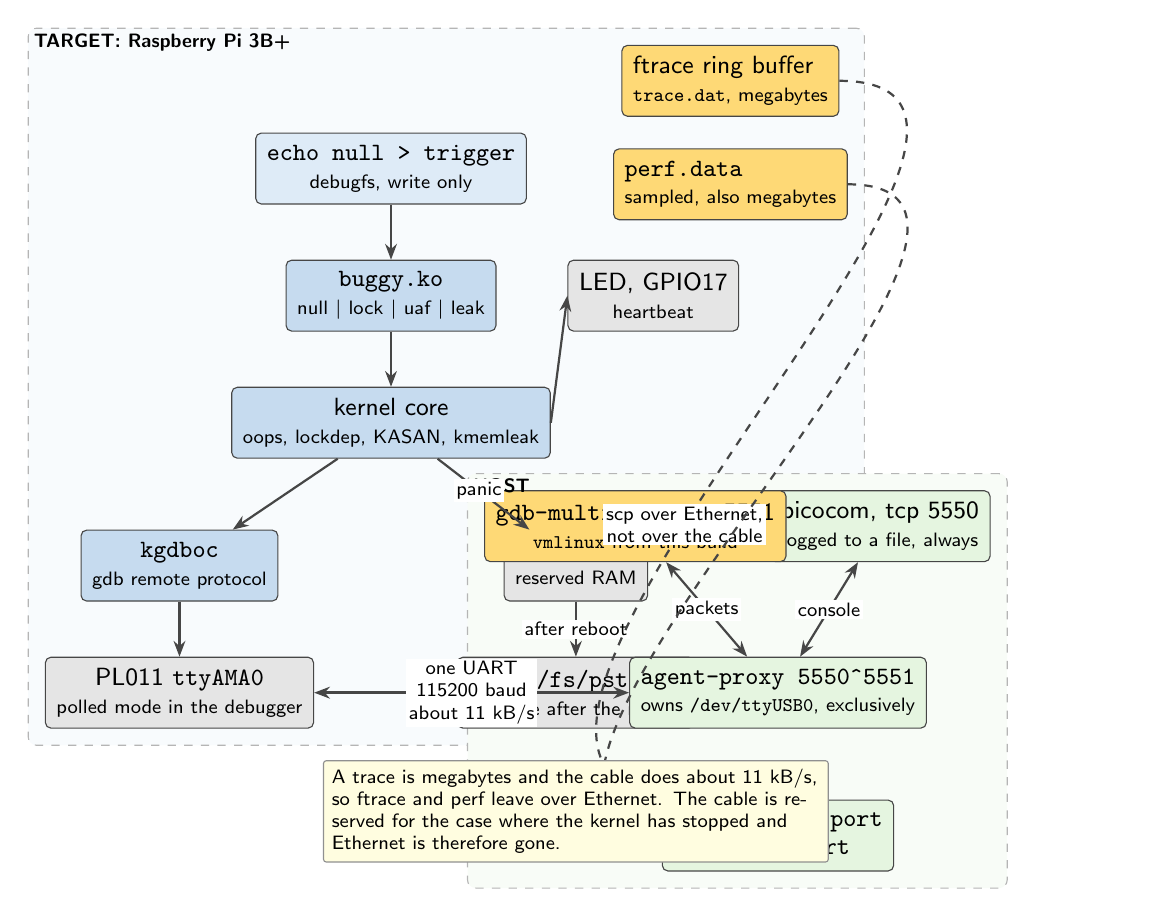
\begin{tikzpicture}[node distance=5mm]

  %% ---------------- target ----------------
  \node[user] (trig) {\texttt{echo null > trigger}\\[-1pt]
                      \scriptsize debugfs, write only};
  \node[kern, below=7mm of trig] (buggy)
       {\texttt{buggy.ko}\\[-1pt]
        \scriptsize null \textbar{} lock \textbar{} uaf \textbar{} leak};
  \node[kern, below=7mm of buggy] (core)
       {kernel core\\[-1pt]
        \scriptsize oops, lockdep, KASAN, kmemleak};

  \node[kern, below left=9mm and -6mm of core] (kgdb)
       {\texttt{kgdboc}\\[-1pt]\scriptsize gdb remote protocol};
  \node[hw, below right=9mm and -6mm of core] (ram)
       {ramoops\\[-1pt]\scriptsize reserved RAM};

  \node[hw, below=7mm of kgdb] (pl011)
       {PL011 \texttt{ttyAMA0}\\[-1pt]\scriptsize polled mode in the debugger};
  \node[hw, below=7mm of ram] (pstore)
       {\texttt{/sys/fs/pstore}\\[-1pt]\scriptsize readable after the reboot};

  % The two instruments that deliberately avoid the cable.
  \node[tool, above right=2mm and 12mm of trig, align=left] (trace)
       {ftrace ring buffer\\[-1pt]\scriptsize \texttt{trace.dat}, megabytes};
  \node[tool, below=4mm of trace, align=left] (perf)
       {\texttt{perf.data}\\[-1pt]\scriptsize sampled, also megabytes};

  \node[hw, right=9mm of buggy, align=center] (led)
       {LED, GPIO17\\[-1pt]\scriptsize heartbeat};

  \begin{scope}[on background layer]
    \node[layer, fill=usercol!20, fit=(trig)(buggy)(core)(kgdb)(ram)(pl011)(pstore)(trace)(perf)(led)] (tgt) {};
  \end{scope}
  \node[layerlabel, anchor=north west] at (tgt.north west)
       {TARGET: Raspberry Pi 3B+};

  %% ---------------- host ----------------
  \node[host, right=40mm of pl011, align=center] (proxy)
       {\texttt{agent-proxy 5550\textasciicircum{}5551}\\[-1pt]
        \scriptsize owns \texttt{/dev/ttyUSB0}, exclusively};
  \node[host, above right=12mm and -20mm of proxy] (term)
       {picocom, tcp 5550\\[-1pt]\scriptsize logged to a file, always};
  \node[tool, above left=12mm and -20mm of proxy] (gdb)
       {\texttt{gdb-multiarch}, tcp 5551\\[-1pt]\scriptsize \texttt{vmlinux} from this build};
  \node[host, below=9mm of proxy, align=center] (reports)
       {\texttt{trace-cmd report}\\[-1pt]\texttt{perf report}};

  \begin{scope}[on background layer]
    \node[layer, fill=hostcol!25, fit=(proxy)(term)(gdb)(reports)] (hst) {};
  \end{scope}
  \node[layerlabel, anchor=north west] at (hst.north west) {HOST};

  %% ---------------- flows ----------------
  \draw[flow] (trig) -- (buggy);
  \draw[flow] (buggy) -- (core);
  \draw[flow] (core) -- (kgdb);
  \draw[flow] (core) -- node[lbl, pos=0.45] {panic} (ram);
  \draw[flow] (kgdb) -- (pl011);
  \draw[flow] (ram) -- node[lbl] {after reboot} (pstore);
  \draw[flow] (core.east) -- (led.west);

  % The one cable. Drawn thickest on purpose.
  \draw[wire] (pl011.east) -- node[lbl, align=center]
       {one UART\\115200 baud\\about 11 kB/s} (proxy.west);

  \draw[bus] (proxy) -- node[lbl] {console} (term);
  \draw[bus] (proxy) -- node[lbl] {packets} (gdb);

  % And the path that is deliberately not the cable.
  \draw[flow, dashed] (trace.east) to[out=0, in=170]
       node[lbl, pos=0.6, align=center] {scp over Ethernet,\\not over the cable} (reports.north west);
  \draw[flow, dashed] (perf.east) to[out=0, in=175] (reports.west);

  \node[umlnote, below=4mm of pstore, align=left, text width=62mm]
       {A trace is megabytes and the cable does about 11 kB/s, so ftrace
        and perf leave over Ethernet. The cable is reserved for the case
        where the kernel has stopped and Ethernet is therefore gone.};

\end{tikzpicture}
\end{document}
